\documentclass[10pt]{article}
\usepackage[margin=3cm]{geometry}
\usepackage{graphicx}
\usepackage{wrapfig}
\usepackage{multirow}
\usepackage{hyperref} 


%%%%%%%%%%%%%%%%%%%%%%%%%%%%%%%%%%%%%%%%%%%%%%%%%%%%%%%%%%%%%%%%%%%%%%%%%%%%%%%%%%%%%

\begin{document}
		\graphicspath{{photos/}}
	\begin{wrapfigure}{r}{3cm}
		\vspace{-20pt}
		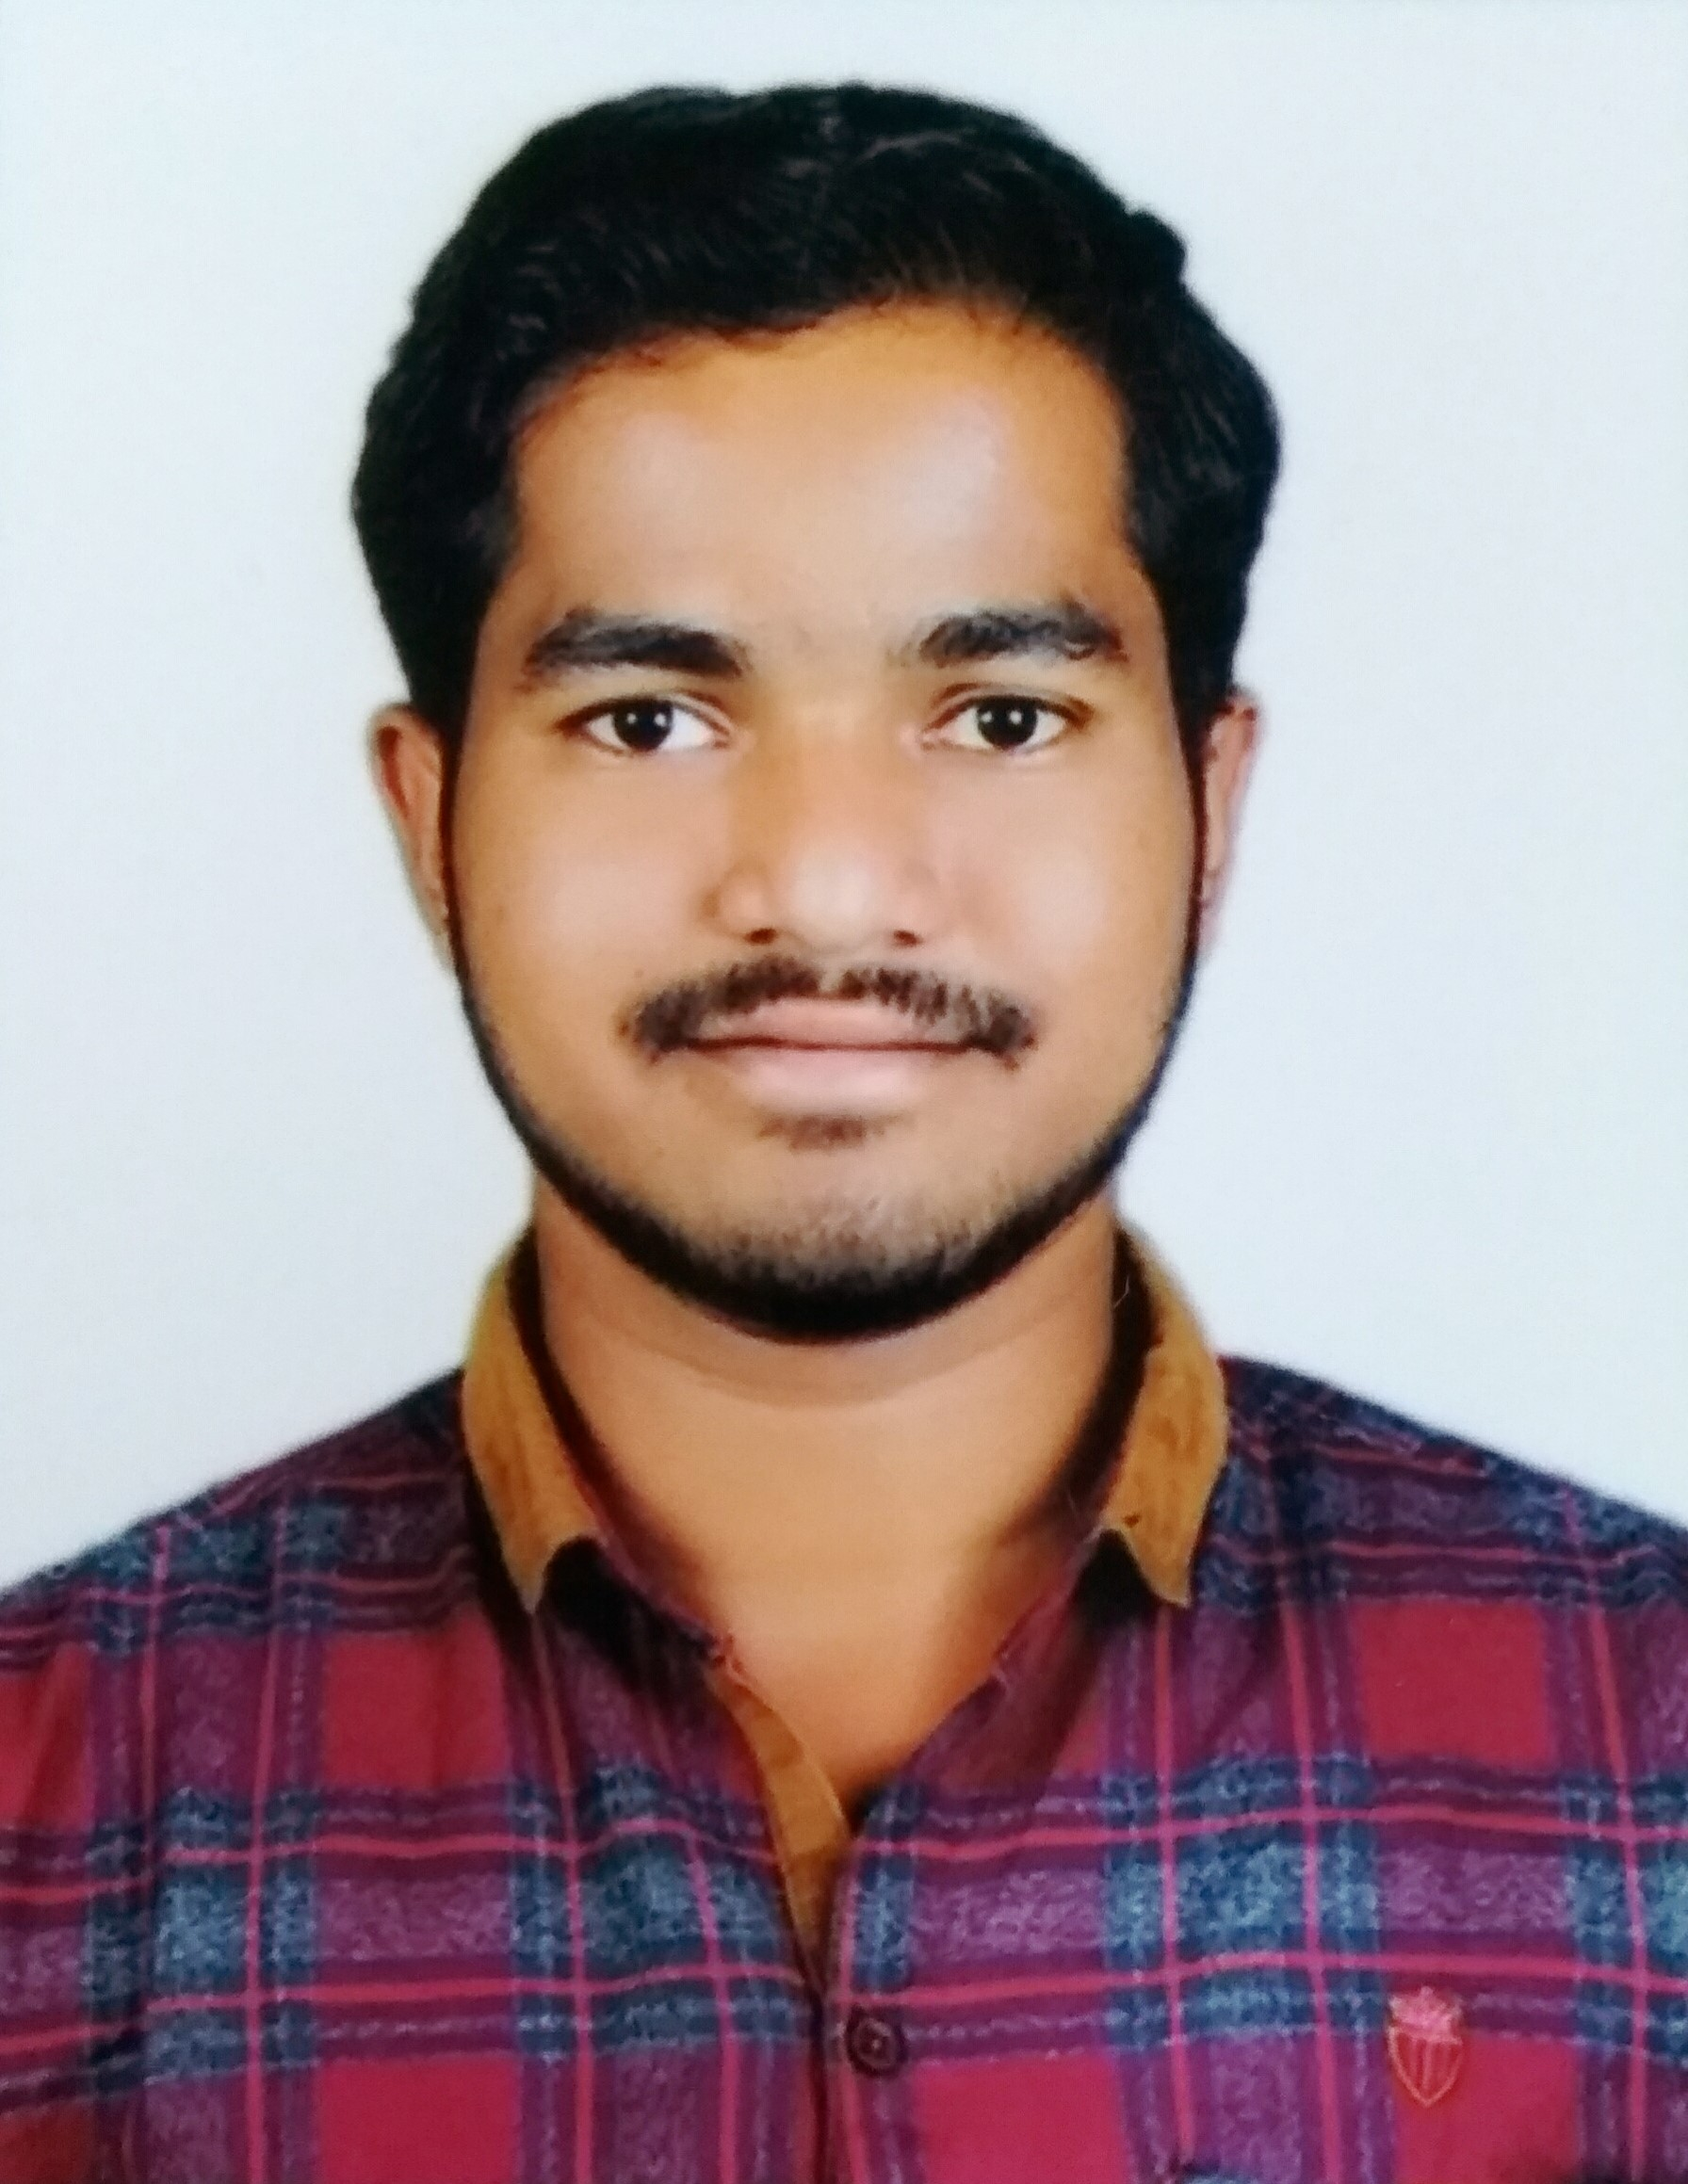
\includegraphics[width=3cm,height=3cm]{photo.jpg}
	\end{wrapfigure}
\textbf{Name:} Mahadev Mishal\\\\
\textbf{Address:} At-vetye, Post-Malgaon Tal-Sawantwadi,\\
Dist-Sindhudurg, Maharastra, PIN: 416510\\
\textbf{conatct No:} 9420886521\\
\textbf{email id:} mishalmahadev500@gmail.com

%%%%%%%%%%%%%%%%%%%%%%%%%%%%%%%%%%%%%%%%%%%%%%%%%%%%%%%%%%%%%%%%%%%%%%%%%%%%%%%%%%%%%
\begin{center}
	\line(1,0){450}
\end{center}

%%%%%%%%%%%%%%%%%%%%%%%%%%%%%%%%%%%%%%%%%%%%%%%%%%%%%%%%%%%%%%%%%%%%%%%%%%%%%%%%%%%%%
\section{Career Objective}
Looking for an internship program where I could learn under working professional to gain knowledge and improvement of my skills by giving some input to the organization.

%%%%%%%%%%%%%%%%%%%%%%%%%%%%%%%%%%%%%%%%%%%%%%%%%%%%%%%%%%%%%%%%%%%%%%%%%%%%%%%%%%%%%
\begin{center}
	\line(1,0){450}
\end{center}

%%%%%%%%%%%%%%%%%%%%%%%%%%%%%%%%%%%%%%%%%%%%%%%%%%%%%%%%%%%%%%%%%%%%%%%%%%%%%%%%%%%%%
\section{Education}
\begin{tabular}{||c|c|c|c|c|c||}
	\hline
	Sr no & class & Institution & board & score&passing year \\
	\hline
	1 &TY& \multirow{3}{*}{ walchand coe sangli} & \multirow{3}{*}{ SUK} & 8.15&on going\\
	2 &SY& && 8.1&2016-17\\ 
	3 &FY& && 8.15&2015-16\\\hline 
	4 &HSC&\multirow{2}{*}{Jawahar Navodaya Vidyalaya Sindhudurg} & \multirow{2}{*}{CBSE}&90.8\%&2013-14\\ 
	5 &SSC& &&90.4\%&2011-12\\
	\hline
	%%%%%%%%%%%%%%%%%%%%%%%%%%%%%%%%%%%%%%%%%%%%%%%%%%%%%%%%%%%%%%%%%%%%%%%%%%%%%%%%%%%%%
\end{tabular}
\begin{center}
	\line(1,0){450}
\end{center}

%%%%%%%%%%%%%%%%%%%%%%%%%%%%%%%%%%%%%%%%%%%%%%%%%%%%%%%%%%%%%%%%%%%%%%%%%%%%%%%%%%%%%
\section{Projects}
\begin{enumerate}
	\item\textbf{ Spotter Snake}
	\begin{itemize}
		\item E-yantra robotics
		competition by IITB.
		\textbf{(Aug 2017-Mar 2018)}
		\item Designing and building of a biomorphic robot that
		resembles a snake capable of traversing different
		terrains and can be used to detect rodents present in
		warehouse.
	\end{itemize}
	\item \textbf{Braille watch}
	\begin{itemize}
		\item Ignited Innovators of India by COE Pune and EATON. \textbf{(Nov 2017-Mar 2018)}
		\item The project is based on braille language used by blind people to read the text. We have used a microcontroller MSP430G2253 and RTC module to actuate the linear actuator which will display time in braille format when requested by user
	\end{itemize}
	\item Line Following Based Multipurpose System for Hospitals:
	\begin{itemize}
		\item India Innovation challenge design contest by Texas Instruments and IIM Bangalore.\textbf{(Quarter final ongoing)}
		\item Our idea is to make a clone of sweeper robot and delivery robot to perform multiple tasks semi-autonomously and autonomously.
	\end{itemize}
	\item \textbf{ Anti-pilferage and anti-adulteration system for fuel road tankers}
	\begin{itemize}
		\item Smart India Hackathon 2017\textbf{(Stage to ongoing)}
		\item System addresses the problem of pilferage and adulteration of fuel tanks en-route from terminals to retail outlets by continuous monitoring of location, level, pressure and temperature parameters with cloud connectivity also ensuring emergency management.
	\end{itemize}
	\item\textbf{ Waveform generator}
	\begin{itemize}
		\item TY B-Tech Mini project\textbf{(Jul 2017-Dec 2017)}
		\item Designed a system to generate waveform using PWM and also using DAC module of LPC2148 microcontroller
	\end{itemize}
\end{enumerate}
%%%%%%%%%%%%%%%%%%%%%%%%%%%%%%%%%%%%%%%%%%%%%%%%%%%%%%%%%%%%%%%%%%%%%%%%%%%%%%%%%%%%%
\begin{center}
	\line(1,0){450}
\end{center}

%%%%%%%%%%%%%%%%%%%%%%%%%%%%%%%%%%%%%%%%%%%%%%%%%%%%%%%%%%%%%%%%%%%%%%%%%%%%%%%%%%%%%
\section{Workshops}
\begin{itemize}
	\item ‘Low Power Microcontroller’ on MSP430 organized by Electronics department, WCE Sangli.
	\item Python organized by WLUG (Walchand Linux User Group).
	\item Proteus professional by ELESA (ELectrinics Engineering Student's Association).
\end{itemize}

%%%%%%%%%%%%%%%%%%%%%%%%%%%%%%%%%%%%%%%%%%%%%%%%%%%%%%%%%%%%%%%%%%%%%%%%%%%%%%%%%%%%%
\begin{center}
	\line(1,0){450}
\end{center}
%%%%%%%%%%%%%%%%%%%%%%%%%%%%%%%%%%%%%%%%%%%%%%%%%%%%%%%%%%%%%%%%%%%%%%%%%%%%%%%%%%%%%
\section{Technical Skills}
\begin{enumerate}
	\item \textbf{Languages:}\\
	\hspace{4cm}      C, Python, C++, Java (novice), VHDL, Verilog, HTML CSS.
	\item \textbf{Microcontroller Known:}\\
	P89V51RD2 (8051), MSP430G2553, MSP432P401R, LPC2148, ATmega 328.
	\item \textbf{Software known}
	\begin{itemize}
		\item \textbf{Circuit simulation and PCB designing:} \\
		Eagle, Altium Proteus professional, Multisim, Webench(TI), PSIM
		\item \textbf{Robotic simulation}\\
		VREP (Virtual Robotics Experimentation Platform)
		\item \textbf{IDE’s}\\
		Energia, u-Vision, Xillinx, CCS, Arduino, Atmel Studio
		\item \textbf{Computational tools:}\\
		MATLAB, LabView
		\item \textbf{3-D designing and animation:}\\
		Autodesk Fusion360, Blender	
	\end{itemize}
\end{enumerate}
%%%%%%%%%%%%%%%%%%%%%%%%%%%%%%%%%%%%%%%%%%%%%%%%%%%%%%%%%%%%%%%%%%%%%%%%%%%%%%%%%%%%%
\begin{center}
	\line(1,0){450}
\end{center}

%%%%%%%%%%%%%%%%%%%%%%%%%%%%%%%%%%%%%%%%%%%%%%%%%%%%%%%%%%%%%%%%%%%%%%%%%%%%%%%%%%%%%
\section{Soft skills}
\hspace{1 cm} Teamwork, Leadership, Workflow Management.

%%%%%%%%%%%%%%%%%%%%%%%%%%%%%%%%%%%%%%%%%%%%%%%%%%%%%%%%%%%%%%%%%%%%%%%%%%%%%%%%%%%%%
\begin{center}
	\line(1,0){450}
\end{center}


\end{document}